\section{Adaptive Landscapes and Evolvability}
\label{sec:evolvability}

\begin{figure}
    \centering
    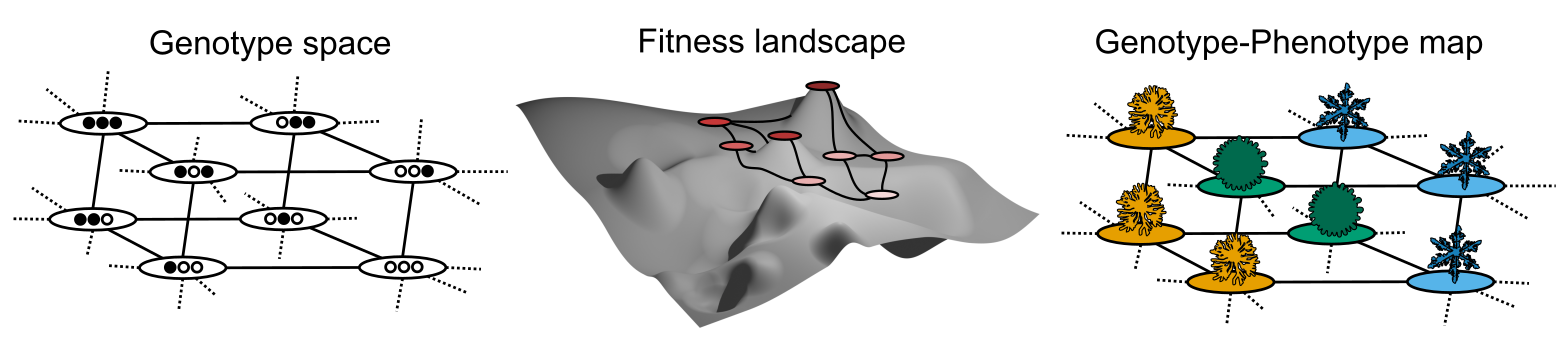
\includegraphics[width=1.0\linewidth]{img/fitness_landscapes.png}
    \caption{%
\textbf{Adaptive Landscapes}.
The \textit{genotype space} (left) is a network of genotypes, with edges connecting genotypes that differ by a single mutation.
A \textit{fitness landscape} (middle) is induced on this space when each genotype is assigned a value denoting its reproductive success in an environment.
Alternatively, the genotypes may be assigned ``phenotypes'' that denote expressed traits, producing a \textit{genotype-phenotype map} (right)
}
\label{fig:fitness_landscapes}
\end{figure}


% \begin{itemize}
% \item \citet{eppstein2016quantifying} use an empirical fitness landscape for $\beta$-lactam antibiotic resistance to quantify deception in evolutionary search, applying evolutionary-computation diagnostics to a biologically grounded mutational graph.
% Their case study shows that real drug-resistance landscapes can exhibit substantial deception, and they introduce a framework for characterizing how landscape topography misleads adaptive walks toward suboptimal peaks.
% \item \citet{schaper2014arrival} argue that strong bias in genotype-phenotype maps --- where some phenotypes are encoded by exponentially more genotypes than others --- systematically channels populations toward ``frequent'' phenotypes regardless of their fitness.
% They show via theory and simulation that this ``arrival of the frequent'' can trap populations on locally suboptimal phenotypes long before selection can act, complicating the standard ``survival of the fittest'' picture of adaptation.
% \item \citet{fragata2019evolution} review recent theoretical and empirical progress in fitness landscape theory, surveying how high-throughput measurements of landscape topography are reshaping understanding of epistasis, ruggedness, and accessibility of adaptive paths.
% The review argues that landscape thinking remains a powerful organizing framework for evolutionary biology, but emphasizes that effective use requires integrating empirical landscape data with population-genetic models of mutation, drift, and selection.
% \item \citet{altenberg1995genome} evelops a theoretical framework in which genome growth via gene duplication interacts with the structure of the genotype-phenotype map to drive the evolution of evolvability.
% He introduces ``constructional selection,'' a second-order process in which newly added genes are retained when their pleiotropic effects tend to produce fitness improvements, thereby biasing genome architecture over time toward representations more conducive to adaptive evolution.
% \item mystery citations \citep{schmitt2003theory,andre2001improvement,bongard2010guarding,pandey2014comparative,crepinsek2013exploration,iwasa2004stochastic,peniston2020environmental,steinberg2016environmental,devos2015breaking}.
% \end{itemize}
%
% While a variety of mechanisms or facets have been brought to evolvability \citep{clune2008natural,hu2010evolvability,altenberg1994evolution,mengistu2016evolvability,riederer2022capturing}.

Evolution differs from random search due to mutational locality, the tendency for a mutant to resemble its parent \citep{maynardsmith1970natural,galvanlopez2011defining,ashlock2012representation,back1996evolutionary,foster2001evolutionary,richter2014fitness}.
This locality defines the geometry of \textit{genotype space} --- the composite arrangement of mutational neighborhoods over all possible genetic sequences \citep{fragata2019evolution,castle2021towards}.
Although classically painted in only one or two dimensions \citep{mcleish2015there,greenbury2022structure,gordon1994evolution,gavrilets1997evolution}, genotype space is more accurately conceptualized as a dense network where each genotype abuts numerous single-mutant neighbors (Figure \ref{fig:fitness_landscapes}, left).

For evolution by natural selection, fitness must vary across genotype space --- creating a \textit{fitness landscape} (Figure \ref{fig:fitness_landscapes}, middle) \citep{pitzer2012comprehensive}.
Where fitness can vary (e.g., ecological or environmental fluctuations \citep{olson2014dynamic,kaplan2008end,dolson2021digital}), a fitness landscape may instead be termed a ``fitness seascape'' \citep{cairns2022strong,mustonen2009fitness}.
Often, it is useful to decompose genotype-fitness relationships to isolate the \textit{genotype-phenotype map} (Figure \ref{fig:fitness_landscapes}, right) \citep{ahnert2017structural,aguilar2018architecture,stadler2003landscapes}.
Biological phenotype (i.e., observable traits) can often be more conveniently and consistently measured than fitness \citep{chen2022environmental,ahnert2017structural,wagner2011pleiotropic,aguilar2018architecture}.
In EC, genotype-phenotype relationships cover indirect encoding techniques, which devise a (typically) lower-dimensional genetic \textit{representation} for hard problems \citep{ashlock2012representation,rothlauf2003redundant,rothlauf2009representations,mitavskiy2003comparing} and defining a ``developmental'' translation into phenotype (i.e., solution) space \citep{stanley2007compositional,stanley2003taxonomy,stanley2009hypercubebased,clune2011performance,kitano1990designing,hornby2002creating}.

Given its strong influence on realized variation, the structure of adaptive landscapes acts as a core determinant of evolutionary outcomes.
Though evolutionary adaptation progresses most efficiently on landscapes that are monotonic and smooth, such conditions rarely occur.
Instead, adaptive landscapes often exhibit extensive \textit{ruggedness} \citep{papkou2023rugged,reidys2001neutrality} and \textit{neutrality} (or near-neutrality) \citep{kimura1983neutral,kimura1991neutral,ohta1992nearly,ohta2002near}.
Even where evolutionary exploration is aided by the mutational dimensionality of large genomes \citep{franke2011evolutionary,greenbury2022structure}, drift effects \citep{reidys2001neutrality,ahnert2017structural,croitoru2022punctuated,galvanlopez2011neutrality,jorg2008neutral,huynen1996smoothness,shackleton2000investigation,huynen1996exploring,amitai2007latent,banzhaf2006evolution,hu2025neutrality,oliveto2017how,wagner2008robustness,wagner2013robustness,masel2010robustness,hu2018neutrality}, and far-reaching jumps via recombination \citep{li2024rapid,doerr2008crossover,fogel1994effectiveness} --- scarcity of available beneficial mutations can nonetheless meaningfully impede adaptation \citep{martin2013multiple,steinberg2016environmental,li2025probability,bank2022epistasis,neidhart2014adaptation,orr2005genetic,bershtein2008advances,van1999neutral}.

A particularly important application of adaptive landscape theory is in the study of \textit{evolvability} --- the capability of a population to produce adaptive genetic variation \citep{payne2018causes,kirschner1998evolvability,wilder2015reconciling,pigliucci2008evolvability}.
\unskip\footnote{%
In addition to local adaptive landscape topology, within-population heterogeneity can also factor in to discussions of evolvability \citep{wilder2015reconciling,houle1992comparing}.
}
Somewhat orthogonal perspectives are brought to evolvability by evolutionary computation and evolutionary biology.
In EC, where alternate genotype-phenotype maps freely originate, it can make sense to consider evolvability as a global property of a given representation \citep{tarapore2015evolvability}.
By contrast, because known life adheres to a common DNA/RNA representation \citep{aguirre2018networked}, counterfactuals are more limited in biology \citep{zhang2015evolution}.
Thus, to evolutionary biologists, evolvability is more naturally framed as a property of localized regions within a large genotype space \citep{wagner2017information,wagner2023evolvability}.

On account of their alternate formulations, biological and computational perspectives on evolvability have exerted strong reciprocal influences \citep{kirschner2017plausibility,dawkins1989evolution,nuodelarosa2017computing,wagner1996perspective}.
In this spirit, we review work across both fields to highlight opportunities --- in both directions --- for further interdisciplinary exchange on evolvability.

\subsection{Evolvability: Mapping-based Perspective}

Owing to the objective-oriented nature of EC, interest in evolvability largely revolves around premature convergence --- problems where evolution gets stuck \citep{crepinsek2013exploration,andre2001improvement,bongard2010guarding,pandey2014comparative,squillero2016divergence}.
In addition to numerous \textit{ad hoc} remedies \citep{ragusa2022augmenting,wang2018population,dang2016selfadaptation,fogel1994introduction,fouskakis2002stochastic,kirkpatrick1983optimization,de2015money,doerr2014impact}, dead-end outcomes can be addressed by rearranging search space.

In this vein, numerous  mechanistic properties of an ``evolvable'' representation that can support such innovation have been proposed \citep{moreno2017evolvability}:
\begin{itemize}
\item \textit{modularity} and \textit{weak linkage}, mechanistic decoupling between phenotypic traits that allows them to vary independently or interact via high-level interfaces \citep{kirschner1998evolvability,downing2015intelligence,kashtan2005spontaneous,kashtan2007varying,wilder2015reconciling,owens2003quest};
\item \textit{degeneracy}, overlapping function among structurally distinct elements which can enhance opportunity for variation \citep{whitacre2010degeneracy,wagner2003evolutionary};
\item \textit{pleiotropy}, the capability for mutation to affect coordinated change across multiple phenotypic traits \citep{rimbault2013derived,cheney2014unshackling};
\item \textit{exploratory growth}, developmental processes that incorporate dynamic feedback to fit structure to context \citep{kirschner1998evolvability,downing2015intelligence},
\item \textit{canalization}, compensatory buffering of phenotypic traits against environmental and genetic perturbation \citep{gibson2004uncovering,paaby2014cryptic};
\item \textit{anisotropy}, biased over-representation of certain phenotypes in genotype space \citep{schaper2014arrival,borenstein2008end,brunusan2025minimal,rohner2025macroevolution,herreralvarez2025structure}; and
\item \textit{symmetry}, bias specifically toward phenotypic structure exhibiting regularity and repetition \citep{coyne1987lack,clune2011performance,tonelli2013relationships,cheney2014unshackling}.
\end{itemize}
Viewing evolvability at the functional level, however, allows a more concise formulation.
\citet{tarapore2015evolvability} define evolvability as capability to innovate by producing variation that is both (1) viable and (2) novel.
\unskip\footnote{%
This framing is also influenced by \citet{kirschner2017plausibility}'s biological theory of facilitated variation.
}
Such capability can be tested using an \textit{evolvability signature} assay, which samples mutational outcomes to describe how strongly fitness constraints penalize phenotypic change.

While these concepts are useful in teasing apart the properties of an existing representation, they do not necessarily imply how to engineer a new one.
This limitation has motivated a slew of recent work in EC that poses genetic representations as a manifold embedding \citep{lehman2023evolution,moreno2018learning,bentley2022evolving,gaier2020discovering,wittenberg2023denoising,bontrager2018deepmasterprints,rodrigueztorrado2020bootstrapping,volz2018evolving,rakicevic2021policy,thakkar2019autoencoder,yosinski2012visually,feng2017autoencoding,stuurman2023approach,li2024generating,song2024morphvae}  --- that is, a lower-dimensional carveout of regions within phenotype space \citep{tenenbaum2000global,roweis2000nonlinear}.

Critically, the shape of such manifolds can, in principle, be learned automatically from training data using unsupervised ML techniques \citep{radford2015unsupervised,turk1991eigenface,white2016sampling,frowd2004evofit}.
Generative Adversarial Networks (GANs), for instance, can be trained from examples to sample over a given manifold \citep{goodfellow2014generative}.
Likewise, bottlenecked and error-correcting autoencoders can learn to distill manifold features and de-noise off-manifold deviations \citep{hinton2006reducing,vincent2008extracting}.
These capabilities lend themselves naturally to genotype-phenotype maps.
Learned mutational operators have also been proposed to similar effect \citep{lehman2023evolution,meyerson2024language}.

\subsection{Evolvability: Neighborhood-based Perspective}

Compared to EC, biological genotype space is staggeringly, exponentially vast \citep{stadler2007fitness,de2014empirical}.
For instance, for even just 20-site RNA strands, upwards of $10^{18}$ mutational paths exist between any pair \citep{greenbury2022structure}.
Despite dense mutational connectivity, the vastness of sequence space affords numerous self-contained neighborhoods \citep{wagner2017information}.
For instance, in a 20-site strand, upwards of 2.59 million sequences exist such that all are at least 5 mutations apart; for 40, 400, and 4,000 site strands, the lower bound on sequences at least 25\% mutually distinct grows to $2.03 \times 10^{11}$, $4.64 \times 10^{97}$, and $9.60 \times 10^{956}$ \citep{gilbert1952comparison,varshamov1957estimate}.
\unskip\footnote{%
As comparison, $10^{88}$ photons have been estimated within the observable universe \citep{dimopoulos1978baryon}.
}

Evolution thus enjoys ample opportunity to exploit variation in local landscape structure in interesting ways \citep{kumawat2024evolution,barnett2025experimental,steinberg2016environmental,gupta2022hostparasite,ferrare2024evolution,pyo2025evolutionary}.
Under a neighborhood-based framing, mutations can be considered ``evolvability enhancing'' if they provide access to later high fitness mutations.
Such mutations can be surprisingly abundant \citep{wagner2023evolvability}, although generality across in biological fitness landscapes remains unexplored \citep{ogbunugafor2023mutations}.
Neighborhood-based evolvability arises also in EC \citep{mengistu2016evolvability,doncieux2020novelty,katona2021quality,lehman2016critical,lehman2013evolvability,reisinger2007acquiring,reisinger2006selecting}, described as \textit{acquired evolvability} \citep{reisinger2005towards}.

Although it is possible to select directly for acquired evolvability in EC \citep{mengistu2016evolvability}, the plausibility of natural evolution favoring genetic neighborhoods with evolvable characteristics hinges on the extent to which --- in addition to instantaneous fitness \citep{watson2016how} --- biases in mutational composition can steer evolution.
While such second-order effects are heavily debated \citep{wagner2021adaptive,akay2016there,keller1999levels,altenberg1995genome,yoshimura1996evolution,yoshimura1991individual,pigliucci2008evolvability}, they have been conclusively demonstrated in specific instances within both biological and computational models \citep{sung2012driftbarrier,wilke2001evolution,pyo2025evolutionary,wagner2021adaptive,akay2016there,keller1999levels,wagner2017information,kumawat2024evolution,barnett2025experimental,steinberg2016environmental,hayden2011cryptic,gupta2022hostparasite,zaman2014coevolution,richter2009detecting,grefenstette1999evolvability}.

While some second-order effects are studied at macroevolutionary timescales (e.g., species selection) \citep{jablonski2008species,stanley1975theory,reznick2009darwin}, particular interest has arisen around the idea that environmental fluctuations acting at shorter, generational timescales \citep{bell2017evolutionary,bell2010fluctuating} can exert lineage selection for evolvability.
Under such conditions, mutations may benefit a lineage directly, or with respect to an environment that is likely to appear in the future \citep{parter2008facilitated}.
For instance, in a changing environment, a high-fitness genotype may be out-competed by genotypes that are lower in fitness, but belong to a lineage that switches quickly between phenotypes adapted to alternate environments \citep{woods2011secondorder}.
Recent work has shown that environmental change pushes populations to these boundaries in genotype space where they can more freely mutate between alternate phenotypes \citep{kumawat2024evolution,barnett2025experimental,kussell2006polymerpopulation,ancel2005evolution}.

Under environmental fluctuations, effective second-order selection requires few local optima remaining stable between conditions --- in other words, the difficulty of co-optimizing alternate fitness landscapes.
To predict adaptive outcomes under shifting conditions, several useful landscape metrics have been recently proposed.
For example, numerous edge-flips in a fitness landscape --- i.e., mutational edges that invert between adaptive and deleterious --- can predict the efficacy of intermittent antimicrobial therapy \citep{chen2024inverted}.
Other work has developed the mutation effect reaction norm (Mu-RN) measure of change in mutational effects and interactions, which can predict when fluctuating selection will favor evolutionary flexibility over immediate fitness \citep{ogbunugafor2022mutation}.

In addition to environmental shifts \citep{king2025fitness,gatenby2020integrating,acar2020exploiting,goulart2013designing}, much other work on adaptive landscapes stems from challenges in evolutionary medicine managing microbial or tumor cell populations during treatment.
For instance, drug resistance mutations have motivated metrics to quantify fitness landscape \textit{deception} acting on a population, according to the fraction of members possessing misleading mutation combinations that provide higher-than-average fitness despite leading away from the global optimum \citep{eppstein2016quantifying}.
Related work has explored how clonal interefence effects driven by the distribution of fitness effect sizes along adaptive trajectories shapes evolutionary outcomes \citep{ogbunugafor2016competition}.

\subsection{Evolvability: Open Questions}

Taken together, evolutionary computation and evolutionary biology paint a more complete picture of evolvability than either can alone.
Natural history proves sophisticated evolvability can emerge with no explicit design, while the extensive challenges encountered by artificial models make clear such evolvability is by no means for granted.

TODO concise but artificial.
Promising work has taken key steps in extending a machine learning framing of evolvability, wherein evolution may ``learn'' from past environments, to mechanisms driven purely by selection and implicit regularization constraints driven by metabolic costs  \citep{kouvaris2017evolution,watson2016how,watson2014evolution}.
Notably, such work has advanced heavily in collaboration with evolutionary computation practitioners \citep{kouvaris2017evolution,szilagyi2020phenotypes,mitchell2025genomic}.
Contemporary developments in machine learning theory remain to be integrated in this framework, however --- such as double descent, which reveals how growth in model size beyond the interpolation threshold can improve, rather than worsen, overfitting \citep{belkin2019reconciling,rocks2022memorizing,nakkiran2021deep}.

More generally, progress is needed towards a systematic taxonomy of second-order selection effects \citep{gajewski2019evolvability,mengistu2016evolvability,hu2010evolvability}.
Ideally, from a biological perspective, such theory would predict under what conditions a population would localize to different boundary genotypes \citep{kussell2006polymerpopulation}.
It is plausible that existing EC selection schemes can already exhibit strong second-order selection for evolvability \citep{hu2010evolvability,doncieux2020novelty,lehman2015enhancing}, which --- along EC's unique experimental tractability --- makes them ideal candidates for such work.
Such collaborations may ultimately help guide effective use of large search spaces with representation optimizing algorithms in EC, to provide better overall results than directly trying to find a good representation \citep{hewlett2008optimization,gajewski2019evolvability,mengistu2016evolvability}.
